\section{Theorie}
\label{sec:Theorie}

%Quantenzahlen
\subsection{Gesamtwellenfunktion und Quantenzahlen}
Die Lösung des Wasserstoffproblems liefert die Wellenfunktion
\begin{equation*}
    \Psi_{n, l, m} (x, y, z) = R_{n, l}(r) \cdot Y_l^m (\vartheta, \varphi) \cdot \chi_{m_s}
\end{equation*}
, welche die Verteilung der Aufenthaltswahrscheinlichkeit eines Elektronens angibt.\\
Die Quantenzahl $n = 1, 2, 3 ...$ wird als Hauptquantenzahl bezeichnet, diese gibt die Elektronenschale bzw. das Energieniveau an zu dem der Zustand des Elektrons gehört.
Die Nebenquantenzahl $l = 0, 1, 2, ..., n-1 $ wird auch Drehimpulsquantenzahl genannt, da dieser nach \autoref{eqn:eigenwert_l} den Eigenwert vom Quadrat des Drehimpulsoperators angibt. 
Um die räumliche Orientierung des Drehimpulses anzugeben, wird die Magnetische Quantenzahl $m = \frac{L_z}{\hbar} = -l, - (l-1), ..., (l-1), l$ verwendet.
Die Spinquantenzahl $s = -\frac{1}{2} , \frac{1}{2}$ gibt den Spin an.
Die Wellenfunktion von Mehrelektronenatomen wird aus dem Produkt der Wellenfunktion einzelner nicht wechselwirkender Teilchen gebildet.
Für die Quantenzahlen gelten die gleichen Definitionen.
\\ \\
Der Bahndrehimpuls und der Elektronenspin stehen wie folgt mit den Quantenzahlen in Relation:
\begin{align}
    |\vec{l}| &= \sqrt{l(l+1)} \hbar \label{eqn:eigenwert_l} \\
    |\vec{s}| &= \sqrt{s(s+1)} \hbar \label{eqn:eigenwert_s}
\end{align}
\FloatBarrier
% jj- und ls-kopplung

%Normaler Zeeman
\subsection{Normaler Zeeman-Effekt}
Wird ein Atom in ein Magnetfeld $B$ gebracht, so spalten sich die $(2l + 1)$ entarteten Spektrallinien in $(2l + 1)$ äquidistante Energieniveaus auf (siehe Abb. \ref{fig:zeeman_aufspaltung}).
Die Aufspaltung der Spektrallinien, die durch das magnetischen Moment des Bahndrehimpuls $l$ \eqref{eqn:eigenwert_l} erzeugt wird, wird als normaler Zeeman-Effekt bezeichnet.
Das Bohr'sche Magneton
\begin{equation}
    \mu_B = \frac{e \cdot \hbar}{2 m_e}
    \label{eqn:magneton}
\end{equation}
gibt im Bohr'schen Atommodell den Betrag des magnetischen Moments eines Elektrons im Grundzustand an.
Hierbei steht $e$ für die Elementarladung, $\hbar$ für das reduzierte Plancksche Wirkungsquantum und $m_e$ für die Ruhemasse des Elektrons.

Der Abstand der Zeeman-Komponenten ist konstant und beträgt
\begin{equation}
    \Delta E = E_{n,l,m} - E_{n,l,m-1} = \mu_B \cdot B \, .
    \label{eqn:energie_dif_normal}
\end{equation}
\\
\begin{figure}
    \centering
    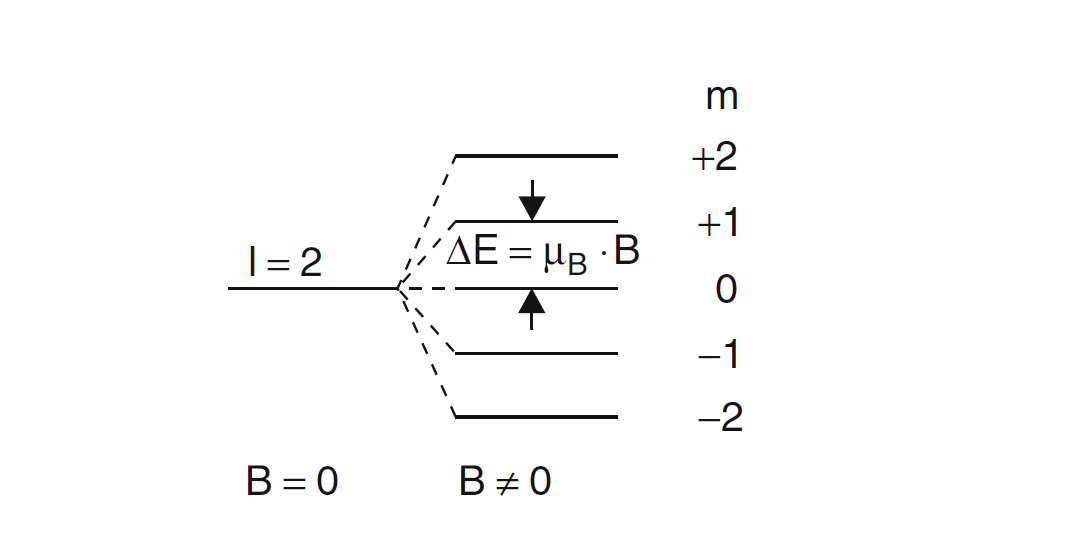
\includegraphics[width=0.6\textwidth]{content/data/zeeman_aufspaltung.png}
    \caption{Schematische Darstellung des Zeeman-Effekts. Die Spektrallinien spalten sich unter Einfluss eines Magnetfeldes auf. \cite[150]{demtroeder}} %ref
    \label{fig:zeeman_aufspaltung}
\end{figure}

Das magnetische Bahnmoment des Elektrons bzw. das magnetische Moment des Drehimpulses
\begin{equation}
    \vec{\mu_l} = -\frac{\mu_B}{\hbar} \cdot \vec{l}
    \label{eqn:magn_moment_l}
\end{equation}
ergibt sich aus dem Bohrschen Magneton $\mu_B$ \eqref{eqn:magneton}, dem reduzierten plankschen Wirkungsquantum $\hbar$ und dem Einheitsvektor $\vec{l}$.
 
\subsection{Emission und Absorption von Licht}
Die Übergangsdipolmomente oder auch Dipolmatrixelemente genannt müssen für einen erlaubten Übergang $E_i \rightarrow E_k$ ungleich null sein.
Daraus lassen sich Auswahlregeln für die Quantenzahlen ableiten.
Für die magnetische Quantenzahl muss $\Delta m = 0$ (linear polarisiertes Licht) oder $\Delta m = \pm 1$ (zirkular polarisiertes Licht) gelten.
Die Übergänge sind in Abb. \ref{fig:uebergaenge} schematisch dargestellt.

Es existieren weitere Auswahlregeln für $l$, $S$ und $J$, diese werden für den Versuch nicht benötigt und daher nicht weiter erläutert.
\\
\begin{figure}
    \centering
    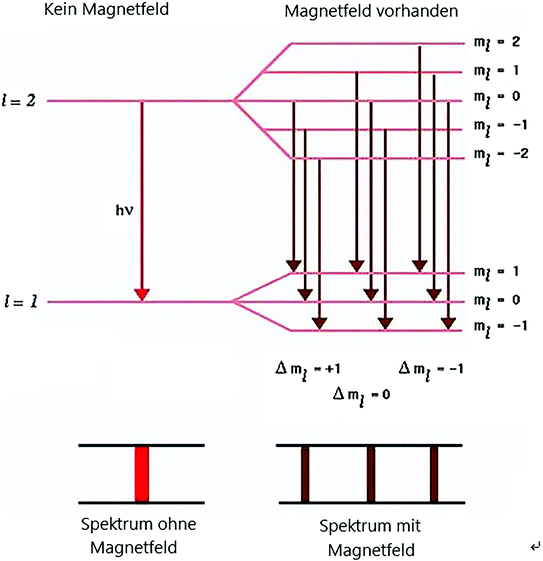
\includegraphics[width=0.6\textwidth]{content/data/uebergaenge_zeeman.png}
    \caption{Schematische Darstellung der Übergänge. \cite{sternspektren}} %ref
    \label{fig:uebergaenge}
\end{figure}
Betrachtet man Emission und Absorption von Licht durch Atome in einem Magnetfeld mit $\vec{B} = B \cdot \vec{z}$ wird folgendes beobachtet:

\begin{itemize}
    \item fällt $\sigma^+$-polarisiertes Licht in $z$-Richtung auf ein Atom, so treten Übergänge mit $\Delta m = +1$ auf
    \item analog dazu treten bei $\sigma^-$-polarisiertem Licht Übergänge mit $\Delta m = -1$ auf
    \item bei der Emission von Photonen, wird entsprechend $\sigma^+ -$ und $\sigma^-$-Licht in Feldrichtung $\vec{z}$ beobachtet
    \item senkrecht zum Magnetfeld werden drei linear polarisierte Komponenten gemessen (2 senkrecht und eine parallel zu $\vec{z}$)
    \item die Spektrallinien werden bei einem Übergang zwischen zwei Zuständen $(n_1,l_1) \rightarrow (n_2,l_2)$ in drei Zeeman-Komponenten aufgespalten: $\sigma^+$, $\sigma^-$, $\pi$ -Polarisation
\end{itemize}
\FloatBarrier

\subsection{Annomaler Zeeman-Effekt}
Der anomale Zeeman-Effekt tritt auf, wenn der Gesamtspin $\vec{S} = \sum_i \vec{s_i}$ eines Atoms ungleich null ist.
Die Aufspaltung der Spektrallinien ist in diesem Fall komplizierter, da der Elektronenspin mit einem magnetischen Moment
\begin{equation}
    \mu_s = -g_s \cdot \frac{\mu_B}{\hbar} \cdot \vec{s}
    \label{eqn:lande_s}
\end{equation}
(analog zum Drehimpuls) verbunden ist.
Dabei wird $g_s$ als (Spin-)Landé-Faktor bezeichnet, wobei $g_s \approx 2$ aus der Dirac-Theorie folgt.
\\
Der Gesamtdrehimpuls $\vec{j} = \vec{l} + \vec{s}$ ist ohne Magnetfeld zeitlich konstant, also behält Richtung und Betrag bei.
Das gesamte magnetische Moment
\begin{align*}
    \vec{\mu_j} &= \vec{\mu_l} + \vec{\mu_s} \\
    &= - \frac{e}{2m_e}(\vec{l} + g_s \vec{s})
\end{align*}
präzediert um $\vec{j}$, da $\vec{s}$ im atomaren Magnetfeld (erzeugt durch die Bahnbewegung des Elektrons) präzidiert.
\\
Die Projektion von $\vec{\mu_j}$ auf $\vec{j}$, auch als das mittlere magnetische Moment bezeichnet
\begin{align*}
    <\mu_j> &= \frac{\mu_j \cdot \vec{j}}{|\vec{j}|}\\
    &= -\frac{e}{2m_e} \left ( \frac{\vec{l} \cdot \vec{j}}{\vec{|j|}} + g_s \cdot \frac{\vec{s} \cdot \vec{j}}{\vec{|j|}} \right )
\end{align*}
wird mithilfe der Produkte $\vec{l} \cdot \vec{j}$ und $\vec{s} \cdot \vec{j}$ wie folgt ausgedrückt:
\begin{align*}
    <\mu_j> &= - \frac{3j(j+1) + s(s+1) - l(l+1)}{2 \cdot \sqrt{j(j+1)}} \mu_B \\
    &= - g_j \cdot \sqrt{j(j+1)} \mu_B \\
    &= - g_j \cdot \frac{\mu_B}{\hbar} \cdot \vec{|j|}
\end{align*}

Der Landé-Faktor
\begin{equation}
    g_j = 1 + \frac{j(j+1) + s(s+1) - l(l+1)}{2j(j+1)}
    \label{eqn:lande}
\end{equation}
kann als Quotient vom gemessenen magnetischen Moments durch den klassisch theoretisch bestimmten Wert betrachtet werden.
Ist nur ein Bahndrehimpuls vorhanden $\vec{j}=\vec{l}$ bzw. nur ein Spinmoment $\vec{j}=\vec{s}$, so beträgt der Faktor $g_j=1$ bzw. $g_j = g_s \approx 2$.
\\
Im folgenden Teil wird die Annahme getroffen, dass das äußere Magnetfeld $\vec{B}$ schwächer als das durch die Bahnbewegung des Elektrons erzeugte Feld ist.
Dann bleibt die Spin-Bahn-Kopplung ($\vec{j}=\vec{l}+\vec{s}$) erhalten und der Betrag des Gesamtdrehimpulses
\begin{equation*}
    |\vec{j}| = \sqrt{j(j+1)} \hbar
\end{equation*}
ist im äußeren Magnetfeld konstant.
Die Richtung ändert sich, aufgrund des magnetischen Moments $\vec{\mu_j} = \vec{\mu_l} + \vec{\mu_s}$, welches ein Drehmoment im Magnetfeld erfährt.
Für die z-Komponente des mittleren magnetischen Moments $<\mu_j>$ kann
\begin{equation*}
    <\mu_j>_z = - m_j \cdot g_j \cdot \mu_B
\end{equation*}
gefolgert werden, wobei $m_j$ halbzahlige Werte im Bereich $-j \leq m_j \leq j$ annehmen kann.
Daraus folgt für die Energie
\begin{align}
    E_{m_j} &= m_j \cdot g_j \cdot \mu_B \cdot \vec{B} + E_0
    \label{eqn:energie_anomal}
\end{align}
, wobei $E_0$ das Energieniveau bei ausgeschaltetem Magnetfeld angibt.
Die Energiedifferenz $\Delta E = E_{m_j} - E_{m_{j-1}}$ zwischen zwei Zeeman-Linien kann nach \autoref{eqn:energie_anomal} bestimmt werden.
Der Landé-Faktor \eqref{eqn:lande} ist abhängig von den Quantenzahlen $j,l$, daher ist die Aufspaltung der Sepktrallinien für die unterschiedlichen Niveaus verschieden.
Um aus den Wellenlängenverschiebungen der Spektrallinien die Landé-Faktoren zu berechnen wird zunächst die Energiedifferenz
\begin{equation*}
    \Delta E = g _\text{ij} \mu _\text{b} B
\end{equation*}
mit
\begin{equation*}
    \Delta E = -h \frac{c}{\lambda^2} \delta \lambda
\end{equation*}
gleichgesetzt.
Die zweite Gleichung ergibt sich aus der Ableitung der Frequenz nach der Wellenlänge, wonach die Gleichung zur Frequenz hin umgestellt wird.
Das Resultat wird nach dem Landé-Faktor umgestellt, was die Gleichung 
\begin{equation}
    g_\text{ij} = \frac{hc \Delta \lambda}{4 \lambda^2 B \mu_\text{B}}
    \label{eq:Lande_Faktor}
\end{equation}
ergibt.
\FloatBarrier

\subsection{Lummer-Gehrcke-Platte}
Die Lummer-Gehrcke-Platte wird zur makroskopischen Untersuchung der Spektrallinien verwendet.
Der Aufbau und Strahlengang kann in Abb. \ref{fig:lummer} betrachtet werden.
Das Licht trifft zuerst auf ein Prisma und wird auf eine planparallele Platte reflektiert.
Nun wird das Licht knapp unter dem Grenzwinkel der Totalreflexion reflektiert, so dass bei jeder Reflexion ein Teil des Licht aus der Platte austritt.
Die Strahlen interferieren nach
\begin{equation*}
    2 \cdot n \cdot d \cdot \cos (\beta) = m \cdot \lambda
\end{equation*}
miteinander, wobei $n$ der Brechungsindex, $m$ die Ordnungszahl der Interferenz, $\lambda$ die Wellenlänge des eintreffenden Lichts, $d$ die Dicke der Platte und $\beta$ den Winkel unter dem das Licht reflektiert wird darstellt.
\begin{figure}
    \centering
    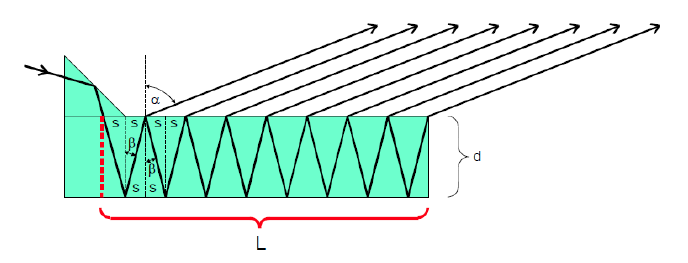
\includegraphics[width=0.8\textwidth]{content/data/lumer_gehrcke_platte.png}
    \caption{Schematische Darstellung des Strahlengangs in einer Lummer-Gehrcke-Platte. \cite[2]{anleitung}} %ref
    \label{fig:lummer}
\end{figure}
\\
Das Dispersionsgebiet ist näherungsweise für große Austrittswinkel $\alpha$ (siehe Abb. \ref{fig:lummer}) mit
\begin{equation}
    \Delta \lambda_D = \frac{\lambda^2}{2d} \frac{1}{\sqrt{n^2 -1}}
    \label{eqn:dispersion}
\end{equation}
gegeben.
Man kann diese Größe als maximale Wellenlängendifferenz zwischen zwei aufgespaltenen Wellenlängen interpretieren, damit sich die verschiedenen Ordnungen nicht überlagern.
\\
Das Auflösungsvermögen lässt sich aus der Länge der Lummer-Gehrcke-Platte $L$, der Wellenlänge $\lambda$ des einfallendes Lichts und dem Brechungsindex $n$ berechnen
\begin{equation}
    A = \frac{\lambda}{\Delta \lambda} = \frac{L}{\lambda} (n^2 - 1) \, .
    \label{eqn:aufloesung}
\end{equation}
\\
\\
Die in diesem Versuch verwendete Lummer-Gehrcke-Platte hat die Maße $d=\SI{4}{\nano\metre}$ und $L=\SI{120}{\milli\metre}$.
Das berechnete Dispersiongebiet $\Delta \lambda_D$ \eqref{eqn:dispersion} und Auflösugsvermögen $A$ \eqref{eqn:aufloesung} für die rote $\lambda = \SI{643,8}{\nano\metre}$ und blaue Linie $\lambda = \SI{480}{\nano\metre}$ ist in Tab. \ref{tab:aufloesung_dispersion} zu finden.

\begin{table}
    \centering
    \caption{Das Dispersionsgebiet $\Delta \lambda_D$ und Auflösungsvermögen $A$ der blauen und roten Spektrallinie.}
    \sisetup{table-format=3.1}
    \begin{tabular}{c c c}
        \toprule
        Linie & $\Delta \lambda_D \,/\, \si{\pico\metre}$ & $A$ \\
        \midrule
        rote & $48,9$ & $209129$ \\
        blaue & $27,0$ & $285458$ \\
        \bottomrule
    \end{tabular}
    \label{tab:aufloesung_dispersion}
\end{table}
\FloatBarrier

\subsection{Termschema für die rote und blaue Linie von Cadmium}
In Abb. \ref{fig:termschema_cd} kann das Termschema zur roten $ ^1 P_1$ $\leftrightarrow$ $^1 D_2$ und blauen $ ^3 S_1$ $\leftrightarrow$ $^3 P_1$ Linie betrachtet werden.
\begin{figure}
    \centering
    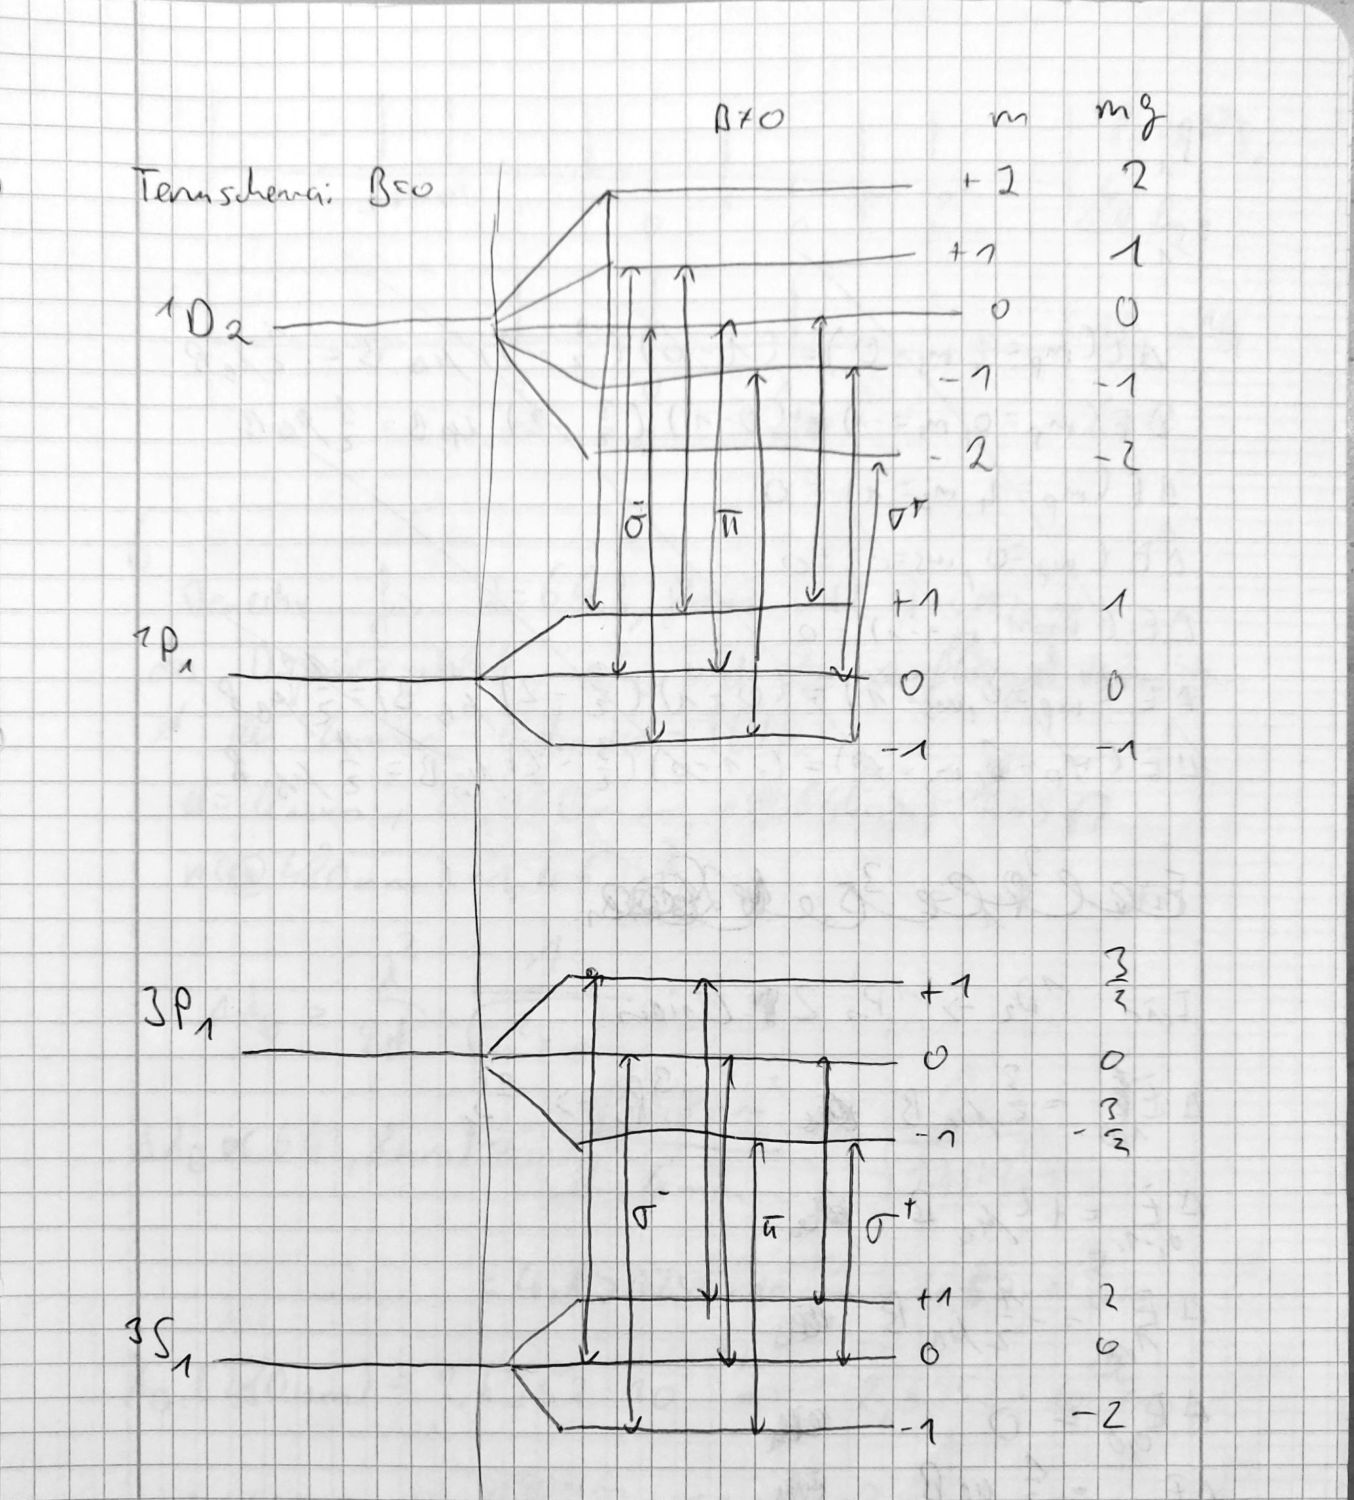
\includegraphics[width=0.8\textwidth]{content/data/termschema_skizze.pdf}
    \caption{Termschema der roten (oben) und blauen Linie (unten) der Cd-Lampe.}
    \label{fig:termschema_cd}
\end{figure}

Zur Berechnung des Landé-Faktor \eqref{eqn:lande} werden $S$ und $L$ nach der Spektroskopischen Notation $^{2S+1}J$ abgelesen.
Aus den berechneten Landé-Faktoren bzw. aus dem Produkt $m \cdot g$ (siehe Abb. \ref{fig:termschema_cd}) kann die Energiedifferenz nach \autoref{eqn:energie_anomal} für die $\sigma-$ und $\pi-$ Linien bestimmt werden.
\\
Die Energiedifferenzen $\Delta E_{i,j} = \left ( m_i g_i - m_j - g_j \right ) \cdot \mu_B B$ ergeben sich für die rote Linie $ ^1 P_1$ $\leftrightarrow$ $^1 D_2$ wie folgt:
\begin{align*}
    \Delta E_{2,1} =  \Delta E_{1,0} = \Delta E_{0,-1} = \mu_B B \,\,\, (\Delta m &= -1) \\
    \Delta E_{1,1} = \Delta E_{0,0} = \Delta E_{-1,-1} = 0 \,\,\, (\Delta m &= 0) \\
    \Delta E_{0,1} =  \Delta E_{-1,0} = \Delta E_{-2,-1} = - \mu_B B \,\,\, (\Delta m &= +1)
\end{align*}
\\
Für die blaue Linie $^3 S_1$ $\leftrightarrow$ $^3 P_1$ folgt:
\begin{align*}
    \Delta E_{1,0} = \frac{3}{2} \mu_B B \,\, \text{und} \,\, \Delta E_{0,-1} = 2 \mu_B B \,\,\, (\Delta m &= -1) \\
    \Delta E_{1,1} = - \frac{1}{2} \mu_B B \,\, \text{und} \,\, \Delta E_{0,0} = 0 \,\, \text{und} \,\, \Delta E_{-1,-1} = \frac{1}{2} \mu_B B \,\,\, (\Delta m &= 0) \\
    \Delta E_{0,1} = -2 \mu_B B \,\, \text{und} \,\, \Delta E_{-1,0} = -\frac{3}{2} \mu_B B \,\,\, (\Delta m &= +1)
\end{align*}
\FloatBarrier

\subsection{Berechnung des Magnetfelds}
Das Magnetfeld muss optimal eingestellt sein, da sich die Linien sonst bei einem zu großen $B$-Feld überlappen.
Wird hingegen eine zu geringe Feldstärke gewählt, so werden die Linien nicht weit genug getrennt.
Nach Gleichung
\begin{equation}
    B = - \frac{\hbar c}{\lambda^2 g_{i,j} \mu_B} \cdot \Delta \lambda_D
\end{equation}
ergeben sich die optimalen Magnetfelder für die jeweiligen $\pi-$ und $\sigma-$Linien.

Die Ergebnisse sind in Tabelle \ref{tab:magnetfelder} zu sehen.
\begin{table}
    \centering
    \caption{Optimale Magnetfeldstärke $B$ für die jeweiligen Spektrallinien.}
    \sisetup{table-format=3.1}
    \begin{tabular}{c r}
        \toprule
        Linie & $B \, / \, \si{\milli \tesla}$ \\
        \midrule
        Rot $\sigma$ & $632,2$ \\
        Blau $\pi$ & $1254,2$ \\
        Blau $\sigma$ & $365,0$ \\
        \bottomrule
    \end{tabular}
    \label{tab:magnetfelder}
\end{table}